\documentclass[article]{IEEEtran}
\usepackage[brazilian]{babel}
\usepackage[utf8]{inputenc}
\usepackage{cite}
\usepackage{geometry}
\usepackage{graphicx}
\usepackage{amsmath}
\graphicspath{{./images/}}
\usepackage{float}
\usepackage[hyphens,spaces]{url}

\begin{document}

%
% paper title
% Titles are generally capitalized except for words such as a, an, and, as,
% at, but, by, for, in, nor, of, on, or, the, to and up, which are usually
% not capitalized unless they are the first or last word of the title.
% Linebreaks \\ can be used within to get better formatting as desired.
% Do not put math or special symbols in the title.
\title{Utilização de fibras ópticas em sistemas de telecomunicação}



% author names and affiliations
% transmag papers use the long conference author name format.

\author{
	Felipe C. S. Santos,
	\and
	Thiago K. Lago
	
\IEEEauthorblockA{Universidade Federal do Rio de janeiro \\ 
	Escola Polit\'{e}cnica \\
	Departamento de Engenharia Eletrônica}
}



\IEEEtitleabstractindextext{
\begin{abstract}

\end{abstract}
\begin{IEEEkeywords}
Telecomunicações, fibras ópticas, optoeletrônica
\end{IEEEkeywords}}



% make the title area
\maketitle

\IEEEdisplaynontitleabstractindextext
As fibras ópticas tem diversas finalidades, sendo uma das mais importantes a utilização em telecomunicações. O avanço das tecnologias de fabricação, modulação e também instrumentação tem tornado cada vez mais viável a utilização das mesmas para transmissões de dados a grandes distâncias com altas taxas de bits. Busca-se através deste paper mostrar o processo de escolha de dimensionamento de uma rede baseada em componentes óticos.
\IEEEpeerreviewmaketitle



\section{Introducão}
\subsection{Elementos do sistema}
\par Qualquer sistema de comunicação pode ser representado pelo diagrama na figura \ref{fig:diagrama-sistema-comunicacao}, este é composto por distintos elementos que possuem as seguintes funções: \cite{FUND_OPT}

\begin{enumerate}
\item \textbf{Fonte:} Responsável pela geração da informação a ser transmitida
\item \textbf{Emissor}: Possui o papel de acoplar a mensagem a um meio de transmissão
\item \textbf{Canal:} É o meio de transmissão em si. Atenua o sinal enviado e insere um ruído. Para comunicação, pode ser o ar, fios ou a fibra óptica.
\item \textbf{Receptor:} Possui a finalidade de tratar a mensagem vinda pelo canal e enviá-la ao destinatário
\item \textbf{Destinatário:} É o destino da mensagem.
\end{enumerate}

\begin{figure}[h]
\label{fig:diagrama-sistema-comunicacao}
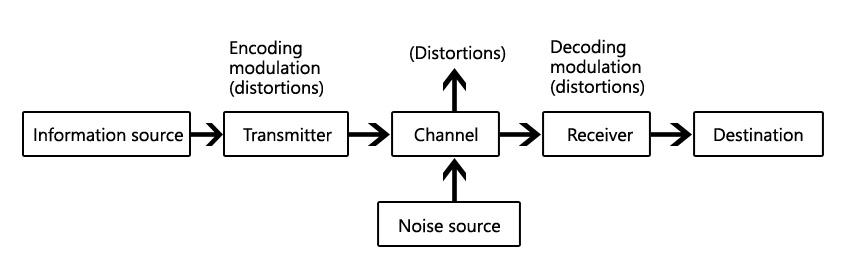
\includegraphics[width=\columnwidth]{communication-system.jpg}
\caption{Diagrama de blocos de um sistema de comunicação}
\end{figure}

Para o caso da fibra óptica, o emissor é uma fonte luminosa, que envia à fibra ópica (o canal) luz. A luz é interpretada no receptor, que pode ser um sensor fotovoltaico. A mensagem agora em pulsos elétricos é enviada ao destinatário e pode ser utilizada como qualquer outra mensagem vinda de um diferente meio de comunicação.
\section{Construção da fibra}
Comentar sobre os materiais que são construídos, as janelas de transmissão, os tipos de dispersão, custo-benefício de cada uma delas.

\section{Componentes óticos}
Comentar sobre alguns componentes óticos utilizados como fbg para filtragem dos sinais e amplificadores ópticos

\subsection{Transmissores ópticos}
Os principais tipos de transmissores são:
\subsubsection{LED}
Possuem como principal vantagem se preço, disponibilidade e confiabilidade. A luz é gerada por emissão espontânea, portanto apenas emitem luz incoerente e com amplo espectro. Este tipo de emissor também não é direcional, portanto apenas pode ser acoplado à fibra multimodo e com baixa eficiência.\cite{TRANSMITTERS}
\subsubsection{Diodos de Laser}
Este tipo de diodo possui uma faixa de preço muito mais elevada que o LED. Também são muito sensíveis à temperatura e precisam estar em um ambiente estável para funcionar de maneira ótima. 
Porém este tipo de transmissor possui uma saída mais direcionada que o LED, aumentando assim sua eficiência no acoplamento de fibras ópticas. Este fato também proporciona o uso de fibras ópticas monomodo, aumentando assim a distância alcançada pelo sistema de comunicação. Os diodos lasers, ao contrario do LED, emitem luz coerente portanto a luz é emitida com apenas uma frequência, diminuindo assim a dispersão modal. \cite{TRANSMITTERS}

\subsection{Receptores ópticos}
O receptor óptico é o elemento responsável por detectar a potência óptica incidente e extrair o sinal dela. É um componente crítico pois geralmente determina a eficiência do sistema, e deve manter boas taxas de razão sinal ruido.\cite{RECEIVER}
\subsection{Amplificadores ópticos}
\par Esta tecnologia permitiu um enorme avanço na utilização de fibras ópticas para comunicação em longas distâncias. Antes dos amplificadores ópticos, eram utilizados repetidores eletrônicos. Estes recuperavam o sinal óptico e transformavam a mensagem em sinal elétrico. Este sinal era então amplificado, filtrado, convertido para sinal óptico e finalmente transmitido para a fibra, agora já amplificado. Apesar de possuírem uma boa eficiência, estes repetidores aumentavam o custo do sistema como um todo. Porque possuem uma eletrônica muito complexa, principalmente para transmissões moduladas em altas taxas.
\par Com o avanço da tecnologia de fabricação das fibras, foi possível a criação de amplificadores ópticos, com eles o processo de amplificação é totalmente realizado no domínio óptico. Tornando desnecessário a utilização de amplificadores regenerativos.
\subsubsection{Amplificadores ópticos semicondutores}
Os amplificadores ópticos semicondutores (SOA) amplificam a luz incidente através de emissão estimulada.


\begin{figure}[h]
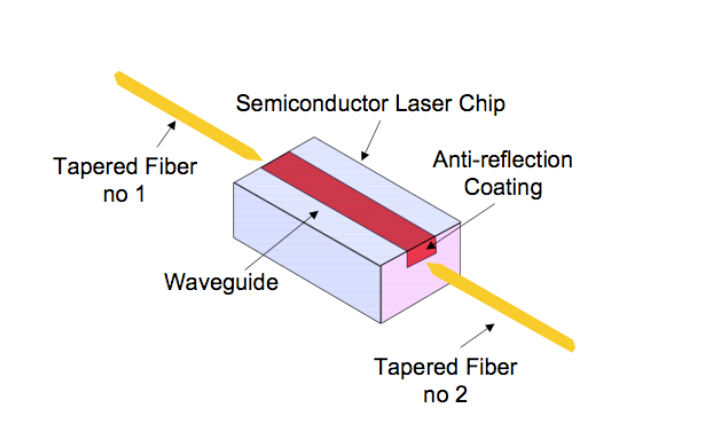
\includegraphics[width=\columnwidth]{soa.jpg}
\end{figure}

A amplificação é obtida bombeando externamente os níveis de energia do material. Para obter apenas a função de amplificação, é necessário proteger o dispositivo contra oscilações próprias, gerando o efeito laser.
Os fótons que passam pela região ativa são estimulados e possuem o mesmo comprimento de onda que o sinal óptico, amplificando assim o sinal óptico durante a passagem pelo dispositivo
\section{Modulações utilizadas}
\subsection{Amplitude Shift Keying (ASK)}
\par A modulação ASK (Amplitude Shift Keying) é um tipo de modulação por intensidade do sinal da portadora, também conhecida por ON-OFF-keying. O sinal é modulado em uma portadora óptica de alta frequência. Na técnica ASK, um sinal de frequência da portadora é adicionado ao sinal da mensagem. Logo uma mensagem com o bit 1, é transmitido um sinal com A W. Enquanto que no bit 0 com 0 W. A modulação ASK é simples de gerar e detectar. No ponto de detecção, a demodulação pode ser realizada facilmente utilizando um detector fotovoltaico, que converte a energia óptica em elétrica, resultando o sinal transmitido.
\par	Para um sistema mais avançado de comunicação, é possível atingir mais de um bit transmitido por símbolo. Isto aumenta a capacidade de transmissão e é conhecido como sinalização multinível. De acordo com a equação $M = 2^N$, M representa o nível do sinal e N o número de bits por segundo e é chamado de M-ary signaling.\cite{MODULATION}
\begin{figure}[hb]
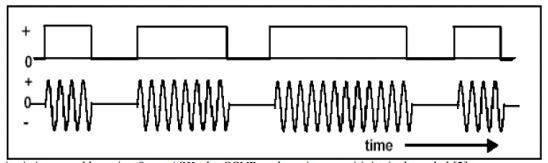
\includegraphics[width=\columnwidth]{ask.png}
\caption{Exemplo de sinal modulado com ASK}
\end{figure}

\subsection{Frequency Shift Keying (FSK)}
\par A modulação FSK é quando a freqüência do laser é trocada entre as duas freqüências. Nesta técnica de modulação. Comparando com a modulação ASK,a complexidade de gerar e receber do sistema aumenta. O formato de modulação diferente baseado no FSK pode ser definido mudando valor do índice de modulação. Uma pequena mudança no índice de modulação resulta em um espectro óptico mais compacto. Em sistemas já implantados, um formato de modulação não pode ser substituído pelo formato de modulação baseado em FSK devido à complexidade do sistema receptor. Nesta técnica, os parâmetros do transmissor e os  parâmetros do receptor devem ser idênticos.\cite{MODULATION}

\begin{figure}[hb]
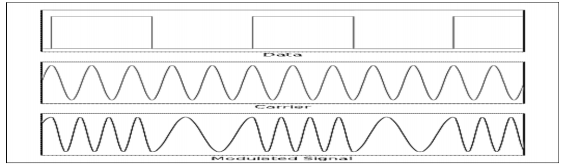
\includegraphics[width=\columnwidth]{fsk.png}
\caption{Exemplo de sinal modulado com FSK}
\end{figure}

\subsection{Phase Shift Keying (PSK)}
\par Phase Shift Keying é a técnica de modulação digital em que a fase da portadora muda, alterando a entrada por senos ou cossenos. Essa modulação possui  dois tipos, a BPSK e QPSK.
\subsubsection{BPSK}
\par Nesta técnica, a portadora senoidal toma duas formas de phase, 0º e 180º.
\subsubsection{QPSK}
\par Nesta técnica, a portadora senoidal pode tomar diversos valores de fase como 0º, 90º, 180º e 270º.

\begin{figure}[h]
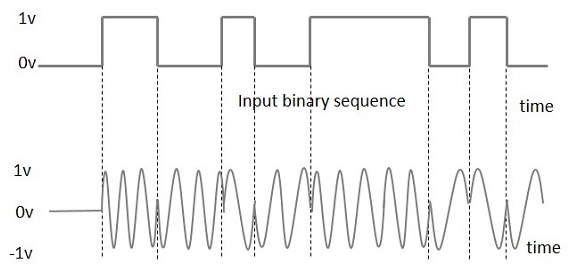
\includegraphics[width=\columnwidth]{psk.png}
\caption{Exemplo de sinal modulado com PSK}
\end{figure}

\subsection{Polarization Shift Keying (PolSK)}
Na modulação PolSK existem dois estados ortogonais de polarização entre o qual o sinal polarizado é mudado para gerar o sinal PolSK. Nesta modulação, o conteúdo do sinal é constante , o que melhora a tolerância não linear e sensibilidade para uma melhor utilização da largura de banda do sistema, a modulação PolSK possui um complexo sistema de geração e detecção de sinais, e também é muito sensível a distúrbios de polarização que podem ocorrer na linha de transmissão.\cite{MODULATION}
\begin{figure}[h]
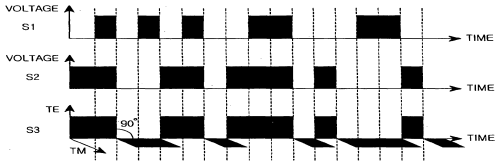
\includegraphics[width=\columnwidth]{polsk.png}
\caption{Exemplo de sinal modulado com PolSK}
\end{figure}

\section{Instrumentros de Medida}
É necessário se preocupar também com a qualidade do sinal recebido e a integridade da fibra óptica. Para isto são utilizados alguns equipamentos que permitem fazer a inspeção das mesmas e analisar o sinal recebido.

Ao instalar uma fibra de grande comprimento, a mesma pode sofrer avarias durante o percurso, prejudicando a recepção do sinal. Outro fator que pode ser determinante na qualidade do sinal recebido é a presença de emendas entre os pedaços das fibras. Existem alguns instrumentos utilizados para resolver este problema. Um deles é o OTDR (\textit{Optical Time Domain Reflectometer}).


\subsection{OTDR}
O \textbf{\textit{OTDR}}  utiliza o efeito de retroespalhamento (\textbf{\textit{backscattering}}) dos raios de luz durante a passagem dos sinais luminosos pela fibra óptica. Assim sendo, torna-se possível medir a atenuação do sinal conforme a distância, assim como visto \cite{FOA}

Esse instrumento possui um laser que emite luz em uma frequência pré-determinada e através da diferença de tempo e da potência do sinal medido após o retroespalhamento é possível determinar a relação entre o sinal recebido e a reflexão em uma dada distância de fibra, assim como visto na figura \ref{fig:otdr_esquematico}. Com isso se torna possível fazer uma inspeção na fibra sem a necessidade de retirar-la do local onde está instalada.


\begin{figure}[H]
	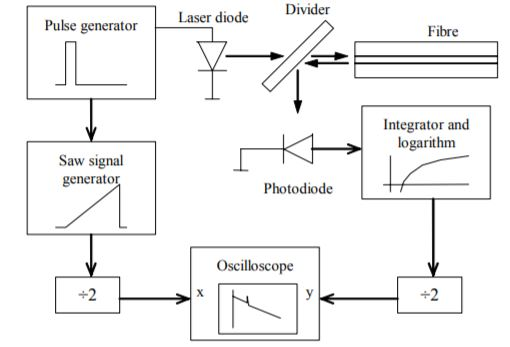
\includegraphics[width=0.5\textwidth]{images/OTDR_esquematico.JPG}
	\caption{Experimento de bancada com OTDR}
	\label{fig:otdr_esquematico}
\end{figure}

O equipamento deve ser conectado conforme a figura [\ref{fig:otdr_teste}], sendo que o cabo de teste pode ter comprimento de alguns quilômetros e ainda sim  pode ser possível realizar a análise com certa clareza. Após uma certa distância, que depende da potência do sinal emitido, da atenuação e reflexão sofrida durante o percurso, o sinal fica num nível comparável ao ruído, conforme visto à esquerda da figura \ref{fig:otdr_teste}:
\begin{figure}[H]
	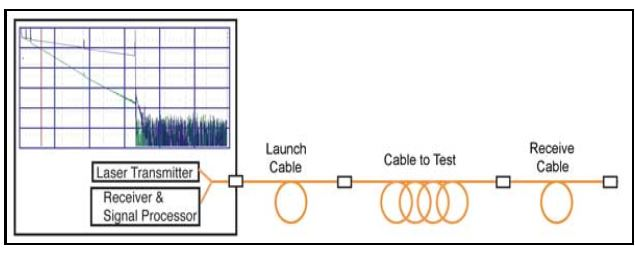
\includegraphics[width=0.5\textwidth]{images/OTDR_teste.JPG}
	\caption{Experimento de bancada com OTDR}
	\label{fig:otdr_teste}
\end{figure}

Uma maneira de aumentar a distância que o sinal chega sem ser muito atrapalhado por ruído é diminuindo o comprimento de onda do laser utilizado na inspeção da fibra. Todavia, isto faz com que a resolução do caminho percorrido diminua, sendo assim, obtêm-se menos informação sobre o caminho percorrido pelo sinal. Cabe ao operador do OTDR ajustar o equipamento de forma a obter o melhor compromisso entre distância e resolução, assim como visto em \cite{OTDR_LAB}.

A inclinação da curva na parte linear indica o coeficiente de atenuação da fibra (db/km). Quanto menor a inclinação, mais longe consegue-se transmitir um sinal até que ele chegue à uma razão sinal ruído (\textbf{SNR}) mínima pré-determinada.

Ao utilizar o equipamento para medir a atenuação do sinal conforme a distância da fibra, pode-se observar um gráfico similar ao visto na figura \ref{fig:OTDR_grafico}:
\begin{figure}[H]
	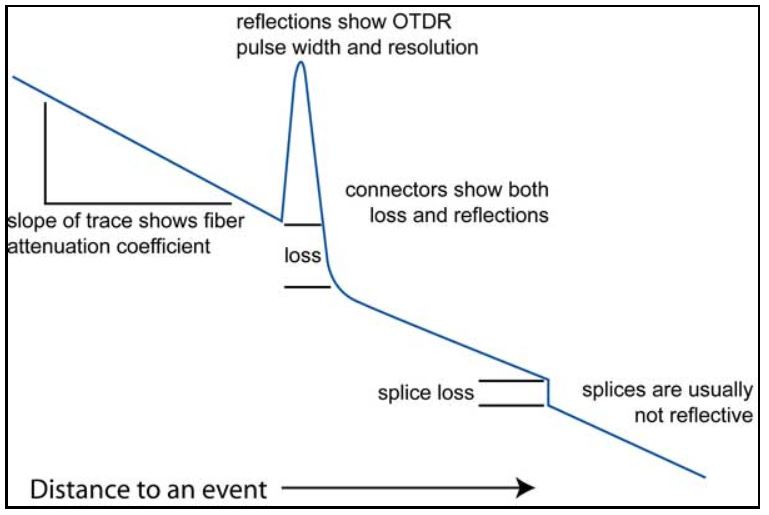
\includegraphics[width=0.5\textwidth]{images/OTDR_grafico.JPG}
	\caption{Experimento de bancada com OTDR}
	\label{fig:OTDR_grafico}
\end{figure} 

Busca-se observar os pontos onde existem descontinuidades na reta de potência do sinal por distância. Estes pontos podem indicar a utilização de um conector mecânico, solda ou até mesmo um rompimento na fibra. Quando a conexão entre fibras é bem feita, a observa-se pouca atenuação no sinal, sendo que a solda bem feita atenua menos que um conector mecânico. Caso observe-se que a inclinação cai bruscamente e o nível do sinal fica próximo ao ruído, pode-se suspeitar de uma fibra rompida ou de uma conexão mal feita.

Existem OTDRs com diferentes finalidades. Antes de fazer a compra do mesmo, necessita-se avaliar o resultado que deseja-se obter com o equipamento. Algumas das perguntas que podem ser feitas são: Há necessidade de ser portátil? Precisa ter bateria? Se precisar, esta deseja-se que esta dure por longo período? A tela precisa ser grande? Qual distância máxima da fibra que desejá-se trabalhar? Qual resolução que se espera nos resultados obtidos? Conforme a pesquisa de preço feito no site mercado livre no dia 30/11/2018 \cite{M_LIVRE}, um OTDR novo pode variar entre R\$3.981, e R\$35.000.

\section{Espectrômetro}


\section{Conclusão}

\bibliographystyle{ieeetr}
\bibliography{citations}

\section{Conclusão}

\end{document}



